\documentclass{article}
\usepackage{doc,url,verbatim,fancyvrb}
\usepackage{pifont}
\usepackage[authoryear]{natbib}
\usepackage[pdftex]{graphicx}
\usepackage{gretl}
\usepackage[letterpaper,body={6.3in,9.15in},top=.8in,left=1.1in]{geometry}
\usepackage[pdftex,hyperfootnotes=false]{hyperref}

\usepackage[utf8]{inputenc}
\DeclareUnicodeCharacter{2212}{-}

% \usepackage[a4paper,body={6.1in,9.7in},top=.8in,left=1.1in]{geometry}

\begin{document}

\setlength{\parindent}{0pt}
\setlength{\parskip}{1ex}
\setcounter{secnumdepth}{1}

% \newenvironment{funcdoc}[1]
% {\noindent\hrulefill\newline\texttt{#1}\par\noindent\hrulefill\par\medskip\par}
% {\bigskip}

\newenvironment{funcdoc}
{\noindent\hrulefill\\[-10pt]}
{\medskip}

\newcommand{\argname}[1]{\textsl{#1}}
\newcommand{\DB}{\textsf{dbnomics}}
  
\title{dbnomics for gretl, version 0.37}
\author{Allin Cottrell \and Jack Lucchetti}
\maketitle

\section{Introduction}
\label{sec:intro}

This package offers an interface to \DB\ for gretl. For
anyone who hasn't yet caught on, \DB\  makes available, in
a uniform manner, a huge number of macroeconomic data series drawn
from many sources around the world---a truly admirable service!

The \DB\ website can be found at \url{https://db.nomics.world/};
interested users are encouraged to visit the site to get a better
sense of what's available. The exact mechanisms whereby \DB\ makes
data available are still under development so some changes can be
expected in future. We will endeavor to keep our package up to date
and will push out updates with gretl snapshots as required.

There are three main layers to the \DB\ ``space,'' as
follows:
\begin{itemize}
\item \textit{Providers}: the various statistical agencies that are
  the primary sources of the data. As of this writing 62 providers
  are included, from the African Development Group to the WTO.
\item \textit{Datasets}: sets of related series offered by a given
  provider. Over 20,000 datasets are available.
\item \textit{Series}: specific time series such as the Bulgarian
  unemployment rate. Hundreds of millions of series are available.
\end{itemize}

A specific series in \DB\ is identified by a triplet
of the form \texttt{provider/dataset/series}, for example
\begin{code}
ECB/IRS/M.IT.L.L40.CI.0000.EUR.N.Z
\end{code}
Here the provider is \texttt{ECB} (the European Central Bank); the
dataset is \texttt{IRS} (interest rate statistics); and the particular
series is ``\texttt{M.IT.L.L40.CI.0000.EUR.N.Z},'' an Italian 10-year
interest rate.

This package provides means of downloading a specific series if you
know its identifying triplet, and also means of navigating the
\DB\ space. There are three ways of accessing the
functionality of the package:
\begin{itemize}
\item Via the gretl commands \cmd{open} and \cmd{data}, as with native
  gretl databases.
\item By means of the gretl GUI.
\item By calling the public functions of the package yourself, in
  command-line or scripting mode.
\end{itemize}
The following three sections expand on these methods in turn.

\section{The \texttt{open} and \texttt{data} commands}
\label{sec:open-data}

To exploit this method you need to know the identifying triplet(s) for
the series you want. Given that, you can initiate \DB\ 
access via the command
\begin{code}
open dbnomics
\end{code}
From this point the \cmd{data} command will target \DB\ 
data until you ``\texttt{open}'' some other data source. So, for
example, you could download the Italian 10-year interest rate
mentioned above in this way:
\begin{code}
data ECB/IRS/M.IT.L.L40.CI.0000.EUR.N.Z
\end{code}

Ah, but what about the name of the series within gretl? The full
triplet is obviously not acceptable as a gretl series-name, and even
its third component won't work since gretl identifiers cannot contain
the dot character. What happens by default is that gretl takes the
third portion of the triplet and squeezes out any illegal characters.
In the case above this would give a name of
\texttt{MITLL40CI0000EURNZ}---not very nice-looking. However, you can
take charge of the naming of the imported series yourself, using the
\option{name} option to the \cmd{data} command, as in
\begin{code}
data ECB/IRS/M.IT.L.L40.CI.0000.EUR.N.Z --name="IT_10yr"
\end{code}
In this case the series will be known to gretl as \texttt{IT\_10yr}.
Note that when you import a series from \DB\ its
descriptive ``label'' starts with the full triplet so you won't lose
that information of record, regardless of the naming of the series.

Note that the \cmd{data} command takes care automatically of several
details, such as for example matching date or adjusting for different
periodicities. For example, the following code snippet will create an
empty monthly dataset and retrieve from \DB\ the monthly index of
industrial production for Portugal, as reported by the ``International
Financial Statistics'' dataset by the International Monetary Fund.
\begin{code}
  nulldata 220
  setobs 12 2007:1
  open dbnomics
  data IMF/IFS/M.PT.AIP_IX --name="pt_ip"
\end{code}
The \cmd{nulldata} and \cmd{setobs} commands used in the above script
will generate a dataset that starts in January 2007 and ends in April
2018, whereas the downloaded series (at the time of this writing)
starts in January 1955 and ends in December 2017, but the \cmd{data}
command puts the numbers in the right place. As for periodicities,
suppose we import the same series into a quarterly dataset, such as
AWM17:
\begin{code}
  open AWM17.gdt --quiet
  open dbnomics
  data IMF/IFS/M.PT.AIP_IX --name="pt_ip"
\end{code}
In this case, the series is also compacted to a lower frequency by
averaging, which is the default behavior of the \cmd{data}
command (see \GUG\ for more details).

\section{dbnomics via the gretl GUI}
\label{sec:dbn-gui}

GUI access to \DB\ is provided in two places (see
Figure~\ref{fig:db-access-1}):
\begin{itemize}
\item Via the \textsf{Databases} item under the \textsf{File} menu in
  the gretl main window.
\item From the gretl databases window (opened by the database icon on
  the toolbar at the foot of the main window): click the ``DB'' icon
  on the toolbar in this window.
\end{itemize}

\begin{figure}[htbp]
  \centering
  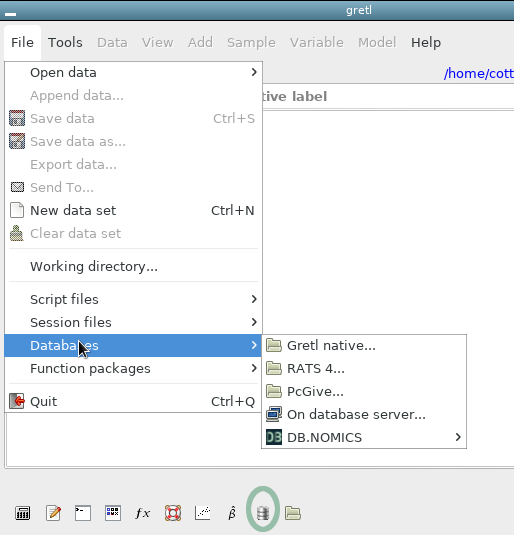
\includegraphics[scale=2.0]{db-access-1}
  \caption{DB.NOMICS access via the File menu or the databases
    button (circled)}
  \label{fig:db-access-1}
\end{figure}

\begin{figure}[htbp]
  \centering
  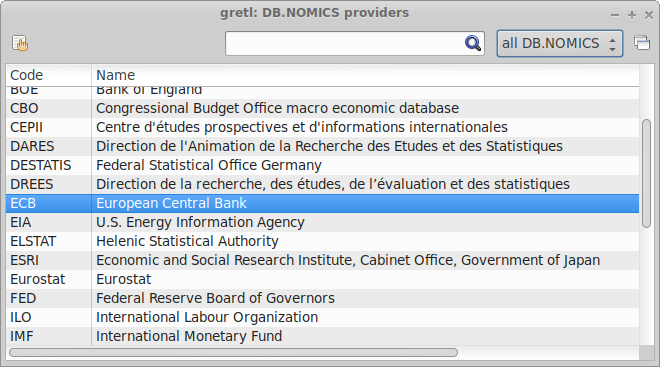
\includegraphics[scale=0.5]{db-access-2}
  \caption{Listing of DB.NOMICS providers}
  \label{fig:db-access-2}
\end{figure}

In both cases you get a little sub-menu with entries
``\textsf{Browse}'' and ``\textsf{Specific series}.'' The latter entry
takes you to a dialog box in which you can enter a series triplet (see
section~\ref{sec:open-data}). The \textsf{Browse} entry takes you to a
window which displays the available \DB\ providers: their codes and
their descriptions (see Figure~\ref{fig:db-access-2}). From here you
have two options:
\begin{itemize}
\item Select a provider and double-click to browse the datasets it
  supplies.
\item In the search box in the top panel of the window, enter a string
  and search all providers for datasets that match your
  specification.\footnote{If you wish to use this facility to find a
    string in the providers window itself, first select ``\textsf{this
      window}'' to the right of the search box, the default being
    ``\textsf{all DB.NOMICS}'' as shown in
    Figure~\ref{fig:db-access-2}.}
\end{itemize}

In each case a \DB\ datasets window will open. With some
providers or searches more datasets will be found than can comfortably
be displayed at once. In that case the toolbar includes buttons that
let you page forward or back through the listing; you should also get
a status message at the foot of the window indicating the current
position in the listing.

From a datasets window two more steps are available:
\begin{itemize}
\item Double-click on a dataset to open a window showing the series it
  contains (or one ``page'' of its full list of series if there are
  too many).
\item In a window showing \DB\ series, double-click to
  activate a particular series. This will give you detailed
  information on the series and allow you to display its values,
  create a time-series plot, or add the series to your gretl dataset.
\end{itemize}

To summarize, there are three layers to gretl's GUI representation of
the \DB\ space:
\begin{enumerate}
\item The providers window (with global search facility)
\item Datasets window (for a given provider, or via search)
\item Series window (for a given dataset)
\end{enumerate}

\section{Public functions}
\label{sec:dbn-funcs}

The package contains several public functions which both subserve the
modes of access described in sections~\ref{sec:open-data} and
\ref{sec:dbn-gui}, and can be called directly by the user.

At this point we just offer an ``as is'' listing of the signatures of
these functions with brief commentary. The finer points are subject to
change; we can expand on them later if there's sufficient
interest.

However, the general guiding principle is that, when you download some
information from \DB, be it a single series or more
complex objects, the metadata are going to be as important as the data
themselves. Therefore, in most cases what you get from the functions
provided by this package are bundles, or arrays of bundles.

For example, the \cmd{dbnomics\_get\_series} function takes as its first
mandatory argument a series code and returns a bundle containing both
the data and the metadata: take the series \texttt{Q.AU.C.A.M.USD.A},
from the ``long series on total credit'' dataset, itself from the Bank
for International Settlements. The code for the dataset is
\texttt{BIS/CNFS}. Therefore, this code snippet
\begin{code}
  b = dbnomics_get_series("BIS/CNFS/Q.AU.C.A.M.USD.A")
  print b
\end{code}
produces the following:
\begin{code}
bundle b, created by dbnomics:
  frequency = 4
  series_name (string, 127 bytes)
  dimensions (bundle)
  dataset_name = long series on total credit
  period = array of strings, length 120
  error = 0
  series_code = Q.AU.C.A.M.USD.A
  indexed_at = 2018-12-13T17:38:15.031Z
  dataset_code = CNFS
  provider_code = BIS
  has_data = 1
  period_start_day = array of strings, length 312
  T = 120
  @frequency = quarterly
  value (matrix: 120 x 1)
\end{code}
The actual data are stored as a column vector, under the key
\texttt{value}; however, there is much more information available to
you: for example, the \texttt{frequency} key equals 4, thus indicating
that the data are quarterly, and so on. If you want to have this
information printed in a more readable way, you'll want to use the
\cmd{dbnomics\_bundle\_print} function, that yields (long lines broken for
readability):
\begin{code}
Series: Q.AU.C.A.M.USD.A
Provider: BIS
Dataset: CNFS (long series on total credit)
Identifier: BIS/CNFS/Q.AU.C.A.M.USD.A
Name: Quarterly – Australia – Non financial sector – Adjusted for
  breaks – Market value – US Dollar – Adjusted for breaks
Dimensions:
  Frequency: 'Q' (Quarterly)
  Borrowers' country: 'AU' (Australia)
  Borrowing sector: 'C' (Non financial sector)
  Lending sector: 'A' (Adjusted for breaks)
  Valuation: 'M' (Market value)
  Type of adjustment: 'A' (Adjusted for breaks)
  Unit type: 'USD' (US Dollar)
------------------------
pd = 4; 120 observations, 1988-Q2 - 2018-Q1
\end{code}

Some functions can be used for retrieving multiple series at once;
therefore, what they return is an \emph{array} of bundles. The
following example fetches two series for two countries from the
``AMECO'' dataset as provided by the European Central Bank. 
\begin{code}
set verbose off
include dbnomics.gfn

bundle spec = null
spec.AME_ITEM = defarray("UBLGE", "OVGD")
spec.AME_REF_AREA = defarray("AUT", "BEL")
bs = dbnomics_get_multiple("ECB", "AME", 20, 0, spec)
dbnomics_bundles_print(bs)
\end{code}
Once the series have been downloaded, a short description of the
resulting array of bundles is obtained by the
\cmd{dbnomics\_bundles\_print} (note the plural) function, and this is
the output (with long lines broken for readability, again):
\begin{code}
Contents of bs:

     Provider  Code                    Description                               
  1: ECB/AME   A_AUT_1_0_0_0_OVGD      Austria - Gross domestic product at 2...
                                       61 observations (pd = 1) [1960:2020]
  2: ECB/AME   A_AUT_1_0_319_0_UBLGE   Austria - Net lending (+) or net borr...
                                       26 observations (pd = 1) [1995:2020]
  3: ECB/AME   A_BEL_1_0_0_0_OVGD      Belgium - Gross domestic product at 2...
                                       61 observations (pd = 1) [1960:2020]
  4: ECB/AME   A_BEL_1_0_319_0_UBLGE   Belgium - Net lending (+) or net borr...
                                       26 observations (pd = 1) [1995:2020]
\end{code}

Note that this package contains several test scripts that
exemplify calls to the functions listed below; this can be found in
the \texttt{examples} subdirectory of the installation
directory. Likely locations for this are as follows (though the paths
may differ by locale and otherwise):

{\small
\begin{tabular}{ll}
  Linux & \texttt{/usr/share/gretl/functions/dbnomics} \\
  Windows & \verb|C:\Program Files\gretl\functions\dbnomics| \\
  Mac & \texttt{/Applications/Gretl.app/Contents/Resources/share/gretl/functions/dbnomics}
\end{tabular}
}

\bigskip

\subsection{List of public functions (in alphabetical order)}

\begin{funcdoc}
\begin{verbatim}
scalar dbnomics_bundle_get_data (const bundle b,
                                 series *x,
                                 bool verbose[0])
\end{verbatim}
Given a bundle obtained by \texttt{dbnomics\_get\_series}, writes the
actual data values (and description) into the series \texttt{x}, which
must exist already and be given in ``pointer'' form. Returns zero on
success, non-zero on error.
\begin{code}
# example
bundle b = dbnomics_get_series("ECB/IRS/M.IT.L.L40.CI.0000.EUR.N.Z")
series IT_10yr = NA
dbnomics_bundle_get_data(b, &IT_10yr)
\end{code}
\end{funcdoc}

\begin{funcdoc}
\begin{verbatim}
void dbnomics_bundle_print (const bundle b,
                            bool print_data[0])
\end{verbatim}
Displays the content of a bundle obtained by
\texttt{dbnomics\_get\_series}. Give a non-zero value for the second
argument to print the actual values, otherwise just the metadata is
shown.
\end{funcdoc}

\begin{funcdoc}
\begin{verbatim}
void dbnomics_bundles_print (const bundles bs)
\end{verbatim}
Displays a concise description of the series contained in an array of
bundles, such as the ones you get from function like
\cmd{dbnomics\_get\_multiple}. For a more detailed printout of the
individual bundles, use \cmd{dbnomics\_bundle\_print}.
\end{funcdoc}

\begin{funcdoc}
\begin{verbatim}
list dbnomics_bundles_to_list(bundles bs, string key[null])
\end{verbatim}
  Creates a list of series from an array of bundles containing series
  data, as returned by functions such as
  \cmd{dbnomics\_get\_multiple}. By default the names of the series
  will be constructed automatically but the second, optional string
  argument can be used to impose a chosen naming scheme: for each
  bundle, if it contains a string value under the specified
  \texttt{key}, that string will be used as the name of the
  corresponding series.
\end{funcdoc}

\begin{funcdoc}
\begin{verbatim}
bundle dbnomics_category_tree (const string provider,
                               bool verbose[0])
\end{verbatim}
  Returns a bundle containing a representation of the ``category
  tree'' for the specified provider. For some providers this tree just
  amounts to a list of datasets but for others it is a hierarchy in
  which related datasets are grouped under one or more levels of
  headings. Each bundle in the tree will have members \texttt{code}
  and \texttt{name}; those that represent groups of datasets rather
  then datasets proper will in addition have a \texttt{children}
  member.
\begin{code}
# example
bundle b = dbnomics_category_tree("BLS")
print b --tree
\end{code}
\end{funcdoc}

\begin{funcdoc}
\begin{verbatim}
bundle dbnomics_dsets_for_provider (const string provider,
                                    bool verbose[0])
\end{verbatim}
  Returns a bundle containing basic information on the datasets
  associated with a given provider, namely two arrays of strings
  holding the codes and names of the datasets respectively.
\begin{code}
# example
bundle b = dbnomics_dsets_for_provider("AMECO")
\end{code}
\end{funcdoc}

\begin{funcdoc}
\begin{verbatim}
series dbnomics_fetch (const string datacode,
                       bool verbose[0])
\end{verbatim}
  This is just a convenience wrapper for
  \texttt{dbnomics\_get\_series} followed by
  \texttt{dbnomics\_bundle\_get\_data}.
\end{funcdoc}

\begin{funcdoc}
\begin{verbatim}
bundles dbnomics_get_cart (const string URL)
\end{verbatim}
This is a convenience function that you can use to select the series
you want via the ``cart'' facility provided by the DB.nomics website.
After choosing the series you want, you have to select the ``Copy API
link'' entry in the ``Download'' menu.

At that point, you can just paste the result into a \app{gretl}
string, and use that as the argument of this function. See the
file \texttt{get\_cart\_example.inp} for an example.
\end{funcdoc}

\begin{funcdoc}
\begin{verbatim}
bundles dbnomics_get_dataset_content (const string provider,
                                      const string dset,
                                      int limit[0::100],
                                      int offset[0])
\end{verbatim}
Returns an array of bundles each containing information on a series
contained in the dataset specified by the \texttt{provider} and
\texttt{dset} codes. The \texttt{limit} and \texttt{offset}
arguments allow ``paging'': retrieve so many results, starting at a
given offset into the full listing.
\begin{code}
# example
bundles B = dbnomics_get_dataset_content("ECB", "IRS", 50, 100)
\end{code}
\end{funcdoc}


\begin{funcdoc}
\begin{verbatim}
bundles dbnomics_get_dataset_dimensions (const string provider,
                                         const string dset,
                                         bool verbose[0])
\end{verbatim}
Returns an array of bundles, with all the ``dimensions'' for a given
dataset, and prints it out if the \texttt{verbose} argument is
nonzero. The dimensions typically contain lists of the different
periodicities of the series contained in the datasets, the
geographical units they refer to, and so on.

Therefore, each resulting bundle will have a key called \texttt{code},
which identifies the dimension, and an array of bundles called
\texttt{values}, describing each dimension via the keys \texttt{code}
and \texttt{label}. For example, the following code
\begin{code}
set verbose off
include dbnomics.gfn

dims = dbnomics_get_dataset_dimensions("ECB", "AME")
code = dims[2].code
vals = dims[2].values
printf "%s\n\n", code
loop i = 1..4 --quiet
    printf "%s - %s\n", vals[i].code, vals[i].label
endloop
\end{code}

returns

\begin{code}
AME_REF_AREA

AUT - Austria
BEL - Belgium
BGR - Bulgaria
HRV - Croatia
\end{code}

\textbf{Note}: This may not work with some providers.
\end{funcdoc}

\begin{funcdoc}
\begin{verbatim}
bundles dbnomics_providers (bool verbose[0])
\end{verbatim}
Returns an array of bundles, one per provider. Each bundle contains
basic info about the provider, notably its dbnomics code under the
\texttt{code} key and its full name under the \texttt{name} key.
\end{funcdoc}

\begin{funcdoc}
\begin{verbatim}
bundles dbnomics_get_multiple (const string provider,
                               const string dset,
                               int limit[0::50],
                               int offset[0],
                               bundle spec[null])
\end{verbatim}
  Returns an array of bundles (defaulting to a maximum of 50), each of
  which contains information (data + metadata) on a series from
  dataset \texttt{provider/dset}.

  The bundle \texttt{spec}, if present, can be used to limit the query
  to certain dimensions. There are two ways to to this:
  \begin{itemize}
  \item you may put a \texttt{mask} key into the bundle, which
    contains a string specially tailored to the specifics of that
    particular dataset. For example, the string
    ``Q.FR+DE+BE.PCPIFBT\_IX'' in the context of the \texttt{IMF/CPI}
    dataset, corresponds to the quarterly price indices for
    ``Alcoholic Beverages, Tobacco, and Narcotics'' in France, Germany
    and Belgium (see the example file
    \texttt{get\_multiple\_example\_via\_mask});
  \item alternatively, you may put into the \texttt{spec} bundle one
    or more string array with the ``dimensions'' for that dataset (see
    the example file \texttt{get\_multiple\_example}).  In order to
    find the dimensions available for a given dataset, use the
    function \cmd{dbnomics\_get\_dataset\_dimensions()}.
  \end{itemize}

\end{funcdoc}

\begin{funcdoc}
\begin{verbatim}
bundle dbnomics_get_series (const string datacode,
                            bool verbose[0])
\end{verbatim}
Returns a bundle containing information on the series specified by
\texttt{datacode}, which must be a \DB\ triplet as
described above.
\begin{code}
# example
bundle b = dbnomics_get_series("ECB/IRS/M.IT.L.L40.CI.0000.EUR.N.Z")
\end{code}
The \cmd{verbose} switch, if true, prints out the actual URL that the
function sends to the \DB\ website, and can be used for debugging purposes.
\end{funcdoc}

\begin{funcdoc}
\begin{verbatim}
bundles dbnomics_search (const string key,
                         const string dset[null],
                         int limit[0::100],
                         int offset[0],
                         bool verbose[0])
\end{verbatim}
  The behavior of this function is dictated by the second parameter
  \texttt{dset}.

  If \texttt{dset} is null, or an empty string, the function
  returns an array of bundles, each holding information on a dataset
  which matches (in some way or other) the \texttt{key} string. If,
  conversely, \texttt{dset} contains a valid dataset representation
  (eg ``\texttt{AMECO/ZUTN}''), then the query will be limited to that
  particular dataset, and the bundles returned will contain the series
  matching the query. See section~\ref{sec:search} below for further
  details.

  The \texttt{limit} and \texttt{offset} argument should in principle
  work to allow paging but as of this writing the \texttt{offset}
  argument has no effect due to a \DB\ bug.
\begin{code}
# example
bundles B = dbnomics_search("interest rates", null, 50)
\end{code}
\end{funcdoc}

\section{Searching \DB}
\label{sec:search}

Given the vast size of the \DB\ space, it's important to
have effective search tools. This is work in progress, but in this
section we illustrate the current state of play. The example below
shows a two-stage search. We first search for relevant datasets across
the whole population of providers then we home in on a particular
dataset and search for relevant series, in each case requesting
verbose results.

\begin{code}
set verbose off
include dbnomics.gfn

# target of search
key = "remittances Iraq"

# search all providers for up to 10 relevant databases
bundles generic = dbnomics_search(key, null, 10, 0, 1)

# search the "WDI" dataset of the World Bank for up to
# 10 relevant series
dataset_code = "WB/WDI"
bundles specific = dbnomics_search(key, dataset_code, 10, 0, 1)
\end{code}

The example produces the following output (long lines broken for
readability):

\begin{code}
Datasets containing "remittances Iraq" (1-5 of 5):

  1: Eurostat.bop_rem6 (42 series)
  2: WB.WDI (5 series)
  3: IMF.BOP (54 series)
  4: CEPII.BOP (54 series)
  5: ECB.BOP (54 series)

Dataset WB/WDI, matching series 1-5 of 5:

BM.TRF.PWKR.CD.DT-IQ: Personal remittances, paid (current US$) -- Iraq
BX.TRF.PWKR.CD.DT-IQ: Personal remittances, received (current US$) -- Iraq
BX.TRF.PWKR.DT.GD.ZS-IQ: Personal remittances, received (% of GDP) -- Iraq
SI.RMT.COST.IB.ZS-IQ: Average transaction cost of sending remittances
  to a specific country (%) -- Iraq
SI.RMT.COST.OB.ZS-IQ: Average transaction cost of sending remittances
  from a specific country (%) -- Iraq
\end{code}

The same search facilities are also available through the GUI: if you
go back to Figure \ref{fig:db-access-2}, you will notice a search text
box at the top. By default, any term you insert will trigger a search
for that term on the whole \DB\ space, like the \cmd{dbnomics\_search}
function with a \texttt{null} second argument. If you want to restrict
the search to a particular dataset instead, you will have to ``click
to'' that particular data set and use the search text box there, like
in Figure \ref{fig:db-access-3}.

\begin{figure}[htbp]
  \centering
  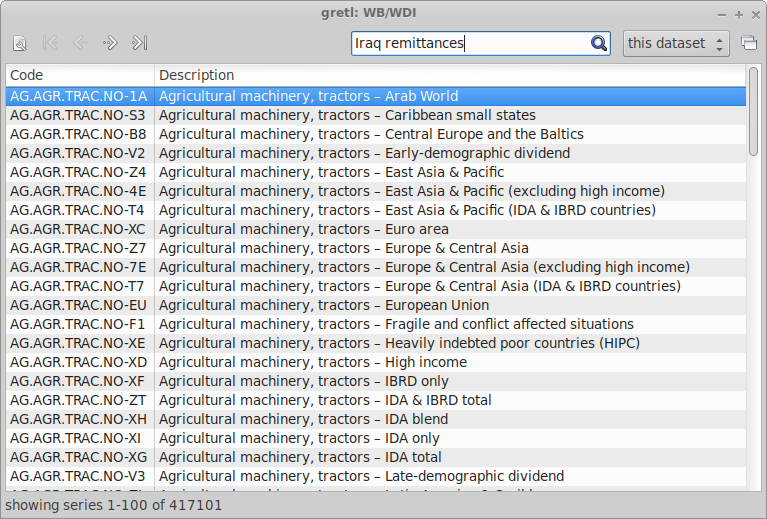
\includegraphics[scale=0.5]{db-access-3}
  \caption{Search within a particular dataset}
  \label{fig:db-access-3}
\end{figure}

\clearpage

\section{Change log}
\label{sec:change-log}

We show below a brief history of changes in the gretl \DB{}
package. Details can be found at
\url{https://sourceforge.net/p/gretl/git/ci/master/tree/addons/dbnomics/}.

\begin{tabular}{llp{.6\textwidth}}
  0.37 & 2020-02-27 & add \texttt{dbnomics\_printer} function \\
  0.36 & 2020-01-25 & add the \texttt{commit\_missing\_periods} flag to our \DB{}
                      requests to ensure we get a full data calendar \\
  0.35 & 2019-07-01 & more work on handling nested JSON arrays \\
  0.34 & 2019-06-26 & work around nested arrays in \DB{} ``dimensions'' info\\
  0.33 & 2019-03-03 & another fix in light of API switch \\
  0.32 & 2019-02-28 & fix minor breakage due to API switch\\
  0.31 & 2019-01-17 & update \DB{} URL\\
  0.3 & 2018-12-23 & switch to version 22 of \DB{} API\\
  0.2 & 2018-11-28 & support downloading of multiple series bundles\\
  0.1 & 2018-06-27 & initial entry as gretl addon
\end{tabular}

\end{document}

%%% Local Variables:
%%% mode: latex
%%% TeX-master: t
%%% End:
